% Options for packages loaded elsewhere
% Options for packages loaded elsewhere
\PassOptionsToPackage{unicode}{hyperref}
\PassOptionsToPackage{hyphens}{url}
\PassOptionsToPackage{dvipsnames,svgnames,x11names}{xcolor}
%
\documentclass[
  authoryear,
  preprint]{elsarticle}
\usepackage{xcolor}
\usepackage{amsmath,amssymb}
\setcounter{secnumdepth}{5}
\usepackage{iftex}
\ifPDFTeX
  \usepackage[T1]{fontenc}
  \usepackage[utf8]{inputenc}
  \usepackage{textcomp} % provide euro and other symbols
\else % if luatex or xetex
  \usepackage{unicode-math} % this also loads fontspec
  \defaultfontfeatures{Scale=MatchLowercase}
  \defaultfontfeatures[\rmfamily]{Ligatures=TeX,Scale=1}
\fi
\usepackage{lmodern}
\ifPDFTeX\else
  % xetex/luatex font selection
\fi
% Use upquote if available, for straight quotes in verbatim environments
\IfFileExists{upquote.sty}{\usepackage{upquote}}{}
\IfFileExists{microtype.sty}{% use microtype if available
  \usepackage[]{microtype}
  \UseMicrotypeSet[protrusion]{basicmath} % disable protrusion for tt fonts
}{}
\makeatletter
\@ifundefined{KOMAClassName}{% if non-KOMA class
  \IfFileExists{parskip.sty}{%
    \usepackage{parskip}
  }{% else
    \setlength{\parindent}{0pt}
    \setlength{\parskip}{6pt plus 2pt minus 1pt}}
}{% if KOMA class
  \KOMAoptions{parskip=half}}
\makeatother
% Make \paragraph and \subparagraph free-standing
\makeatletter
\ifx\paragraph\undefined\else
  \let\oldparagraph\paragraph
  \renewcommand{\paragraph}{
    \@ifstar
      \xxxParagraphStar
      \xxxParagraphNoStar
  }
  \newcommand{\xxxParagraphStar}[1]{\oldparagraph*{#1}\mbox{}}
  \newcommand{\xxxParagraphNoStar}[1]{\oldparagraph{#1}\mbox{}}
\fi
\ifx\subparagraph\undefined\else
  \let\oldsubparagraph\subparagraph
  \renewcommand{\subparagraph}{
    \@ifstar
      \xxxSubParagraphStar
      \xxxSubParagraphNoStar
  }
  \newcommand{\xxxSubParagraphStar}[1]{\oldsubparagraph*{#1}\mbox{}}
  \newcommand{\xxxSubParagraphNoStar}[1]{\oldsubparagraph{#1}\mbox{}}
\fi
\makeatother


\usepackage{longtable,booktabs,array}
\usepackage{calc} % for calculating minipage widths
% Correct order of tables after \paragraph or \subparagraph
\usepackage{etoolbox}
\makeatletter
\patchcmd\longtable{\par}{\if@noskipsec\mbox{}\fi\par}{}{}
\makeatother
% Allow footnotes in longtable head/foot
\IfFileExists{footnotehyper.sty}{\usepackage{footnotehyper}}{\usepackage{footnote}}
\makesavenoteenv{longtable}
\usepackage{graphicx}
\makeatletter
\newsavebox\pandoc@box
\newcommand*\pandocbounded[1]{% scales image to fit in text height/width
  \sbox\pandoc@box{#1}%
  \Gscale@div\@tempa{\textheight}{\dimexpr\ht\pandoc@box+\dp\pandoc@box\relax}%
  \Gscale@div\@tempb{\linewidth}{\wd\pandoc@box}%
  \ifdim\@tempb\p@<\@tempa\p@\let\@tempa\@tempb\fi% select the smaller of both
  \ifdim\@tempa\p@<\p@\scalebox{\@tempa}{\usebox\pandoc@box}%
  \else\usebox{\pandoc@box}%
  \fi%
}
% Set default figure placement to htbp
\def\fps@figure{htbp}
\makeatother





\setlength{\emergencystretch}{3em} % prevent overfull lines

\providecommand{\tightlist}{%
  \setlength{\itemsep}{0pt}\setlength{\parskip}{0pt}}



 
\usepackage[]{natbib}
\bibliographystyle{elsarticle-harv}


\usepackage{gb4e}
\noautomath
% \usepackage[inline]{glossaries}
\usepackage{leipzig}
% \makeglossaries
\usepackage{typgloss}
\usepackage{setspace}
\makeatletter
\@ifpackageloaded{caption}{}{\usepackage{caption}}
\AtBeginDocument{%
\ifdefined\contentsname
  \renewcommand*\contentsname{Table of contents}
\else
  \newcommand\contentsname{Table of contents}
\fi
\ifdefined\listfigurename
  \renewcommand*\listfigurename{List of Figures}
\else
  \newcommand\listfigurename{List of Figures}
\fi
\ifdefined\listtablename
  \renewcommand*\listtablename{List of Tables}
\else
  \newcommand\listtablename{List of Tables}
\fi
\ifdefined\figurename
  \renewcommand*\figurename{Figure}
\else
  \newcommand\figurename{Figure}
\fi
\ifdefined\tablename
  \renewcommand*\tablename{Table}
\else
  \newcommand\tablename{Table}
\fi
}
\@ifpackageloaded{float}{}{\usepackage{float}}
\floatstyle{ruled}
\@ifundefined{c@chapter}{\newfloat{codelisting}{h}{lop}}{\newfloat{codelisting}{h}{lop}[chapter]}
\floatname{codelisting}{Listing}
\newcommand*\listoflistings{\listof{codelisting}{List of Listings}}
\makeatother
\makeatletter
\makeatother
\makeatletter
\@ifpackageloaded{caption}{}{\usepackage{caption}}
\@ifpackageloaded{subcaption}{}{\usepackage{subcaption}}
\makeatother
\journal{Cognition}
\usepackage{bookmark}
\IfFileExists{xurl.sty}{\usepackage{xurl}}{} % add URL line breaks if available
\urlstyle{same}
\hypersetup{
  pdftitle={Sensitivity to within-experiment statistics: A case from Turkish agreement attraction},
  pdfauthor={Utku Turk},
  pdfkeywords={keyword1, keyword2},
  colorlinks=true,
  linkcolor={blue},
  filecolor={Maroon},
  citecolor={Blue},
  urlcolor={Blue},
  pdfcreator={LaTeX via pandoc}}


\setlength{\parindent}{6pt}
\begin{document}

\begin{frontmatter}
\title{Sensitivity to within-experiment statistics: A case from Turkish
agreement attraction \\\large{Within-experiment statistics in agreement
attraction} }
\author[1]{Utku Turk%
\corref{cor1}%
}
 \ead{utkuturk@umd.edu} 

\affiliation[1]{organization={University of Maryland, College
Park, Linguistics},addressline={Marie Mount Hall},city={College
Park},postcode={20742},postcodesep={}}

\cortext[cor1]{Corresponding author}

        
\begin{abstract}
Surface level does not affect it, but within-experiment statistics
effect the findings.
\end{abstract}





\begin{keyword}
    keyword1 \sep 
    keyword2
\end{keyword}
\end{frontmatter}
    

\section{Introduction}\label{introduction}

Speakers often rely on additional sources of information when processing
sentences, including distributional expectations about forms and tasks,
as well as the overall composition of an experimental session (e.g., the
ratio of fillers to critical items). Recent work has demonstrated that
such task-specific factors can substantially modulate reading and
judgment behavior
\citep{LauraMalsbug24, ArehalliWittenberg2021, HammerlyEtAl2019, LogacevVasishth2016}.
One line of research has used the agreement-attraction phenomenon to
probe the heuristics that influence sentence processing. Agreement
attraction refers to cases in which a verb erroneously agrees with a
nearby noun rather than the true subject, giving rise to so-called
grammaticality illusions in both production and comprehension
\citep{BockMiller:1991, PearlmutterGarnseyBock:1999}.

\begin{exe}
\ex[*]{\label{og}The key to the cabinets are rusty.} 
\end{exe}

Agreement errors in sentences like (\ref{og}) have been treated either
as a failure of feature reconcilation or a failure of memory encoding.
The former set of accounts explain these errors as a by-product of how
number feature of a phrase is calculated in real-time
\citep{BockMiller:1991, EberhardEtAl2005, HammerlyEtAl2019}. For
example, \citet{EberhardEtAl2005} argue that depending on conceptual
number, morphophonological number marking, or syntactic dependencies
within a phrase, speakers assign a probabilistic number value to
phrases. The errors arise when additional plurality features from
different sources end up contributing to the final number representation
of a phrase. On the other hand, the latter set of accounts claim that
the initial representation is not erroneous, but speakers are sometimes
unable to correctly retrieve the controller
\citep{WagersEtAl:2009, Dillon2013a}. For example,
\citet{WagersEtAl:2009} argue that the parser normally check the
agreement relation by retrieving the relevant chunk in memory using the
retrieval cues provided by the agreement probe. In sentences like (1),
speakers occasionally retrieve the incorrect element due to the fact
that neither nouns fully match the relevant cues.

However, both group of accounts generally are underspecified in terms of
how meta-linguistic information should be integrated to the
inter-sentential dependency mechanisms. Recently, a growing literature
have been testing how different types of additional sources that are
independent of the linguistic information affects these errors. Recent
experiments show that even small changes in task expectations can alter
attraction patterns. For example, \citet{LauraMalsbug24} found that
varying the practice structure and task demands (reading vs.~judgment)
affected reading times at the verb in sentences as in (\ref{malsburg}).
In a series of high-powered self-paced reading tasks, they found that
when participants answered a comprehension question after each trial,
reading times at the verb `admires' did not differ between
(\ref{malsburg-singer}) and (\ref{malsburg-singers}). However, when
participants were asked to judge grammaticality instead, they spent more
time reading the verb `admires' in (\ref{malsburg-singers}), suggesting
that processing mechanisms can change depending on the expected task.

\begin{exe}
\ex \label{malsburg}
\begin{xlist}
\ex \label{malsburg-singer} The singer that the actor openly admires apparently received broad international recognition.
\ex \label{malsburg-singers} The singers that the actor openly admires apparently received broad international recognition.
\end{xlist}
\end{exe}

A related set of findings came from \citet{HammerlyEtAl2019}. They
challenge long-standing assumption that the agreement errors only
surfaced in ungrammatical sentences such as (\ref{og}), but not in
grammatical sentences as in (\ref{og-g}). It has been repeatedly shown
that a plural noun increased participants' likelihood to erroneously
judgme ungrammatical sentences as grammatical; however, participants
rarely misidentified grammatical sentences as ungrammatical even when
there is an attractor. \citet{HammerlyEtAl2019} showed that similar
effect surfaced in grammatical sentences when participants' a priori
expectations about the experiment is altered. They manipulated the
instructions and the number of ungrammatical in an experiment so that
participants expected to see more ungrammatical sentences than
grammatical sentences. With reduced bias towards grammaticality, they
found that the presence of a plural nearby noun affected how speakers
completed ungrammatical sentences (\ref{og}) and grammatical sentences
(\ref{og-g}) \citep[see][ for acceptability]{Turk2022}.

\begin{exe}
\ex[]{\label{og-g}The key to the cabinets is rusty.}
\end{exe}

Another set of meta-linguistic information that comes from form-driven
task strategies. Attraction effects is argued to be sensitive how
similar the attractor is to a possible agreement controller.
\citet{HartsuikerEtAl2003}, for example, showed that participants made
agreement errors more often when the preambles contained two NPs that
are not marked distinctively (\ref{ger-amb}) compared to cases where the
attractor is distinguishable solely using the form (\ref{ger-dist}).

\begin{exe}
\ex \label{ger}
\begin{xlist}
\ex \label{ger-amb}
\gll Die Stellungnahme gegen ie Demonstration-en\\
the.F.NOM.SG position against the.F.ACC.PL demonstration-PL\\
\glt `The position against the demonstrations' 
\ex \label{ger-dist}
\gll Die Stellungnahme zu den Demonstration-en\\
the.F.NOM.SG position on the.F.DAT.PL demonstration-PL\\
\glt `the position on the demonstrations' 
\end{xlist}
\end{exe}

However, the most striking evidence comes from work by
\citet{Slioussar2018}, who showed that surface form can sometimes
override abstract features in Russian. Exploiting the syncretism between
singular genitives and nominative plurals---a pattern absent in plural
genitives---she found that participants made more production and
comprehension errors and showed faster reading times in sentences like
(\ref{rus-gen-pl}) than in (\ref{rus-gen-sg}). She argued that, rather
than accessing abstract case features, readers relied on surface-level
cues that were easier to retrieve.

\begin{exe}
\ex \label{rus}
\begin{xlist}
\ex \label{rus-gen-sg}
\gll Korobka dlya kraski byla/*byli \ldots \\
box.F.SG.NOM for paint.GEN.SG$_{\neg NOM.PL}$ be.PST.F.SG/*be.PST.F.PL \\
\glt `A box for the paint(s) was/*were \dots'
\ex \label{rus-gen-pl}
\gll Korobka dlya krasok byla/*byli \ldots \\
box.F.SG.NOM for paint.GEN.PL$_{\neg NOM.PL}$ be.PST.F.SG/*be.PST.F.PL \\
\glt `A box for the paint(s) was/*were \dots'
\end{xlist}
\end{exe}

\begin{itemize}
\tightlist
\item
  Form-based influences. in some languages, surface-form similarity can
  exacerbate attraction or even drive illusions on its own.
\item
  Cite \citet{Slioussar2018} and related Russian work: case syncretism
  between nominative plurals and genitive singulars increased attraction
  or slowed reading, suggesting reliance on form-based heuristics rather
  than abstract case features.
\item
  Cite Chromy and checz data. tell it is not very consistent.
\end{itemize}

Building on these observations, we utilize Turkish as a testing ground
to examine how surface-form overlap influences agreement processing and
whether exposure to different kinds of distractors modulates attraction.

\begin{itemize}
\tightlist
\item
  Previous attraction findings in Turkish
\item
  Prior work has reported typical attraction effects with
  genitive-marked nominal attractors, showing higher acceptance of
  ungrammatical plural-verb sentences.
\item
  However, no work has directly tested whether verbal plural morphology
  can induce similar illusions, or how mixing different attractor types
  within an experiment affects the magnitude of attraction.
\end{itemize}

Turkish provides an especially informative case because both nominal and
verbal plural markers are realized with the same morpheme, --lAr, yet
only nominal plurals bear the syntactic features required for agreement.
This allows us to ask whether participants rely on surface-form
similarity or on abstract feature representations when evaluating
agreement.

\begin{itemize}
\tightlist
\item
  Morphological properties
\item
  Turkish marks number on both nouns and verbs using the identical
  plural morpheme --lAr.
\item
  Only nominal plurals introduce number features that can agree with the
  verb; verbal --lAr expresses verbal agreement but is not a potential
  controller.
\item
  Because of this homophony, Turkish allows form-overlap and
  feature-mismatch to be disentangled experimentally.
\end{itemize}

In our first experiment, we test whether plural marking on a verbal
distractor---which is morphologically identical but syntactically
irrelevant---can elicit attraction. In the second experiment, we combine
these verbal distractor conditions with standard nominal attractor
conditions to assess how their co-occurrence affects participants'
judgments. If attraction effects reflect flexible, context-sensitive
processing, the inclusion of verbal distractors should dilute or
eliminate the illusion typically observed with nominal attractors.

Together, these experiments extend previous findings on agreement
attraction and task sensitivity in two key ways. First, they show that
surface-level overlap---even when morphologically identical---does not
by itself produce agreement attraction, indicating that participants
rely on abstract morphosyntactic features rather than phonological
forms. Second, they reveal that participants are not only influenced by
the global structure of an experiment (such as the proportion of fillers
or grammatical items) but also by the presence of other condition types
within the same task. In other words, attraction effects are attenuated
when competing, non-attracting conditions are included, suggesting that
agreement processing is dynamically tuned to the statistical context of
the experiment itself.

\subsection{Experimental logic and
predictions}\label{experimental-logic-and-predictions}

\begin{itemize}
\item
  Goal 1: test whether purely form-based overlap (verbal --lAr) elicits
  attraction.
\item
  Prediction: if attraction is driven by form, verbal plural distractors
  should yield higher ``acceptable'' rates for ungrammatical plurals.
\item
  Alternative: if attraction depends on abstract features, no effect of
  verbal --lAr should appear.
\item
  Goal 2: test whether the co-occurrence of different attractor types
  modulates attraction.
\item
  Prediction: if participants adapt to the distribution of conditions,
  adding verbal distractors (which share the plural form but lack
  agreement features) should attenuate or eliminate the
  nominal-attractor illusion.
\item
  Summary: These experiments jointly test whether agreement attraction
  in Turkish reflects shallow form matching or feature-based computation
  that is sensitive to the statistical context of the task.
\end{itemize}

\section{Experiment 1: Testing Form-Driven
Processing}\label{experiment-1-testing-form-driven-processing}

\subsection{Participants}\label{participants}

We recruited 80 undergraduate students to participate in the experiment
in exchange for course credit. All participants were native Turkish
speakers, with an average age of 21 (range: 18 -- 31). The experiment
was carried out following the principles of the Declaration of Helsinki
and the regulations concerning research ethics at Bogazici University.
All participants provided informed consent before their participation
and their identities were completely anonymised.

\subsection{Materials}\label{materials}

We used 40 sets of sentences like (\ref{exp}), in which we manipulated
(i) the number of the attractor and (ii) the number agreement on the
verb. Both plural markings were marked with the suffix -ler/-lar, while
the singular number and singular agreement were marked by its absence.

\begin{exe}
\ex \label{exp}
\begin{xlist}
\ex[]{\label{ss}
\gll Tut-tuğ-u aşçı mutfak-ta sürekli zıpla-dı.\\
hire-NMLZ-POSS cook[NOM] kitchen-LOC non.stop jump-PST\\
\glt `The cook they hired$_{sg}$ jumped$_{sg}$ in the kitchen non-stop.'}
\ex[*]{\label{sp}
\gll Tut-tuğ-u aşçı mutfak-ta sürekli zıpla-dı-lar.\\
hire-NMLZ-POSS cook[NOM] kitchen-LOC non.stop jump-PST-PL\\
\glt `The cook they hired$_{sg}$ jumped$_{pl}$ in the kitchen non-stop.'}
\ex[]{\label{ps}
\gll Tut-tuk-lar-ı aşçı mutfak-ta sürekli zıpla-dı.\\
hire-NMLZ-PL-POSS cook[NOM] kitchen-LOC non.stop jump-PST\\
\glt `The cook they hired$_{pl}$ jumped$_{sg}$ in the kitchen non-stop.'}
\ex[*]{\label{pp}
\gll Tut-tuk-lar-ı aşçı mutfak-ta sürekli zıpla-dı-lar.\\
hire-NMLZ-PL-POSS cook[NOM] kitchen-LOC non.stop jump-PST-PL\\
\glt `The cook they hired$_{pl}$ jumped$_{pl}$ in the kitchen non-stop.'}
\end{xlist}
\end{exe}

All sentences were adapted by previous studies in Turkish agreement
attraction \citep{LagoEtAl2019, TurkLogacev2020}. Sentences started with
a complex subject NP like `tuttukları aşçı' `the cook they hired,' in
which the nominalized relative clause functioned as the attractor, and
the head noun were bare. Because the plural marking on nominals is not
optional and the head noun was singular, absent of -lar, in all
conditions, sentences with plural verb agreement were ungrammatical. To
inhibit participants from forming a task-related strategy in which they
deemed the sentence ungrammatical upon seeing a plural verb, half of our
fillers included plural grammatical verbs, while the other half included
singular ungrammatical verbs.

\subsection{Procedures}\label{procedures}

The experiment was run online, using the web-based platform Ibex Farm
\citep{Drummond2013}. Each experimental session took approximately 25
minutes to complete. Participants provided demographic information and
gave informed consent to participate in the experiment. They then
proceeded to read the instructions and were given nine practice trials
before the experiment began.

Each trial began with a blank screen for 600 ms, followed by a
word-by-word RSVP presentation of the sentence in the center of the
screen, followed by a prompt to indicate their acceptability judgment.
Sentences were presented word-by-word in the center of the screen in 30
pt font size, at a rate of 400 ms per word. Participants saw a blank
screen for 100 ms between each word, and to see the next item, they
needed to press the space key. Participants were asked to press the key
P to indicate that a sentence is acceptable and Q to indicate that the
sentence is unacceptable. They were instructed to provide judgments as
quickly as possible. During the practice, but not during the experiment,
a warning message in red font appeared if they did not respond within
5,000 ms.

Participants saw 40 experimental and 40 filler sentences. Experimental
sentences were distributed among four different lists according to a
Latin-square design. Every participant saw one version of the experiment
with a specific list and one item per condition.

\subsection{Analysis and Results}\label{analysis-and-results}

\pandocbounded{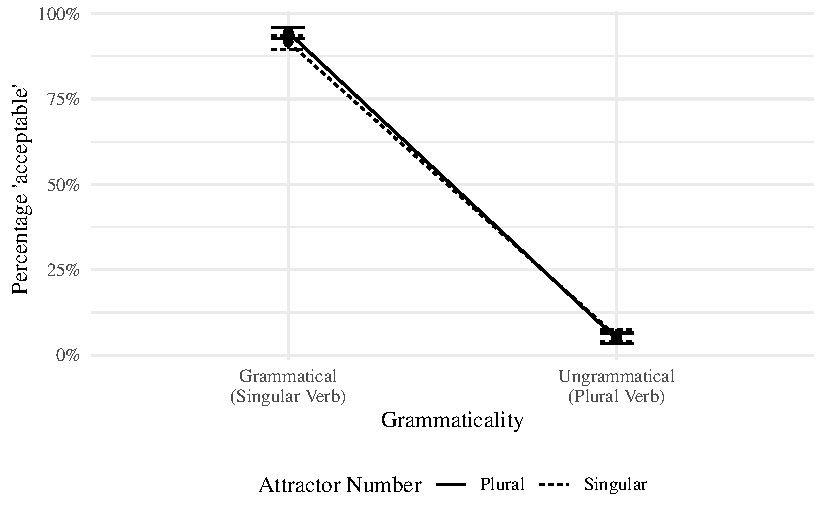
\includegraphics[keepaspectratio]{paper_files/figure-pdf/exp1-plot-1.pdf}}

\begin{itemize}
\tightlist
\item
  Goal: determine if surface plural forms (verbal -lAr) elicit
  illusionary agreement.
\item
  Participants: 80 Turkish speakers (Boğaziçi undergraduates).
\item
  Design: 2 × 2 (Grammaticality × Attractor Number).
\item
  Materials: relative-clause verbs as attractors; same surface
  morphology as nominal plurals.
\item
  Procedure: speeded acceptability judgments, 1500 ms deadline.
\item
  Analysis: Bayesian probit GLM (brms); random intercepts/slopes by
  subject/item.
\item
  Results:

  \begin{itemize}
  \tightlist
  \item
    High filler accuracy (\textgreater{} .9).
  \item
    No difference in ungrammatical sentences between plural vs singular
    attractors.
  \item
    Posterior coefficients near 0; 95 \% CIs within ROPE.
  \end{itemize}
\item
  Discussion:

  \begin{itemize}
  \tightlist
  \item
    No evidence for form-driven guessing.
  \item
    Participants rely on abstract number features, not phonological
    similarity.
  \end{itemize}
\end{itemize}

\section{Experiment 2: Testing Within-Experiment Statistical
Sensitivity}\label{experiment-2-testing-within-experiment-statistical-sensitivity}

\subsection{Participants}\label{participants-1}

We recruited 118 undergraduate students to participate in the experiment
in exchange for course credit. All participants were native Turkish
speakers, with an average age of 20 (range: 18 -- 32). The experiment
was carried out following the principles of the Declaration of Helsinki
and the regulations concerning research ethics at Bogazici University.
All participants provided informed consent before their participation
and their identities were completely anonymised.

\subsection{Materials}\label{materials-1}

The same materials were used with Exp1. We added items from
TurkLogacev2024 as an additional condition.

\subsection{Procedures}\label{procedures-1}

The same procedure with Experiment 1 was used.

\subsection{Analysis and Results}\label{analysis-and-results-1}

\begin{itemize}
\tightlist
\item
  Goal: test whether attraction changes when both attractor types occur
  in one experiment.
\item
  Participants: 95 Turkish speakers.
\item
  Design: 2 × 2 × 2 (Grammaticality × Attractor Number × Attractor Type
  {[}nominal vs verbal{]}).
\item
  Procedure \& analysis: same as Experiment 1.
\item
  Results:

  \begin{itemize}
  \tightlist
  \item
    Attraction replicated for nominal attractors (Δ ≈ 0.07).
  \item
    Verbal attractors again showed null effect.
  \item
    Global decline in yes-responses relative to earlier studies →
    participants became more conservative.
  \end{itemize}
\item
  Discussion:

  \begin{itemize}
  \tightlist
  \item
    Exposure to verbal conditions reduced attraction magnitude overall.
  \item
    Indicates participants adapt to statistical properties of the task.
  \item
    Aligns with learning-based cue-weighting accounts (Haskell et
    al.~2010).
  \end{itemize}
\end{itemize}

\section{General Discussion}\label{general-discussion}

\begin{itemize}
\tightlist
\item
  Synthesis:

  \begin{itemize}
  \tightlist
  \item
    No evidence for surface-form matching; effects are feature-based.
  \item
    Attraction magnitude changes with condition distribution → adaptive
    tuning.
  \end{itemize}
\item
  Interpretation:

  \begin{itemize}
  \tightlist
  \item
    Supports an adaptive parser sensitive to within-experiment
    statistics.
  \item
    Challenges ``shallow'' or ``good-enough'' accounts that attribute
    attraction to phonological overlap.
  \end{itemize}
\item
  Broader implication:

  \begin{itemize}
  \tightlist
  \item
    Agreement processing is flexible and probabilistic; illusions arise
    from learned cue validity.
  \end{itemize}
\item
  Limitations:

  \begin{itemize}
  \tightlist
  \item
    Syntactic depth asymmetry (verbal attractors more embedded).
  \item
    Need future designs equating structure (e.g., embedded-object
    attractors).
  \end{itemize}
\item
  Conclusion:

  \begin{itemize}
  \tightlist
  \item
    Turkish attraction effects arise from abstract feature retrieval not
    surface level shallow form-matching.\\
  \item
    The evaluation of abstract features are modulated by distributional
    learning within the experiment.
  \end{itemize}
\end{itemize}

\section*{References}\label{references}
\addcontentsline{toc}{section}{References}

\newcommand{\doi}[1]{\href{http://dx.doi.org/#1}{http://dx.doi.org/#1}}
\begingroup
\raggedright
\singlespacing

\renewcommand{\bibsection}{}
\bibliography{bibliography.bib}

\endgroup





\end{document}
